\chapter{Contribution}\label{sec:contribution}

This thesis shall be understood as an extension to the works of Evermann et al. \cite{evermann2016} and Schönig et al. \cite{schoenig2018}, both of which were presented in the previous section. The two works have demonstrated the applicability of LSTM neural networks in Predictive Process Monitoring, but have left out the general perspective on the sequence prediction problem. Furthermore, the impact of adding engineered features to the training data was not investigated.\\

The thesis introduces said general perspective through the adaption of the approach of Shibata et al. \cite{shibata2016bipartite}. Their bipartite network architecture as well as the engineered SP-2 features have shown extraordinary performance in the SPiCE competition \cite{web:spice}. This transfer is made under the hypothesis that a case can exhibit properties similar to grammatical rules. Sub-sequence information as proposed by Klinkmüller et al. \cite{klinkmuller2018reliablemonitoring} are considered as an alternative to the SP-2 features. These sub-sequences are mined with PrefixSpan \cite{pei2001prefixspan}.

The two implementations are henceforth referred to as SP2 for the bipartite architecture using SP-2 features and PFS for the bipartite architecture using sub-sequence information mined with PrefixSpan. They are compared to the performance of implementations that mimic Evermann et al. and Schönig et al. Where original performance statistics were published, these are used additionally. The BPIC2011 \cite{BPIC2011} and BPIC2012 \cite{BPIC2012} datasets are used and preprocessed differently as per each approach.\\

The performance of the four different approaches is evaluated along different dimensions, which are explained at the end of this chapter.

\section{Contrasting the compared approaches}
A contribution to current research is the direct comparison of differently designed networks that solve the same prediction problem. \autoref{fig:architectures} shows the four network architectures which are contrasted in \autoref{chap:evaluation}. In the following descriptions, $n$ denotes the number of neurons needed to read the input, while $m$ denotes the number of neurons needed to produce the one-hot-encoded next-activity output.\\

\autoref{fig:evermann-architecture} showcases the ANN architecture used by Evermann et al. \cite{evermann2016}. It has been reverse-engineered from the publicly available code-base \cite{web:evermann} in collaboration with Jörg Evermann. The network itself receives the input data in dictionary-encoded form so that it can be processed by the embedding layer. The embedding produces a 500-dimensional output, which is fed through two LSTM layers which also apply a dropout of $20\%$. Finally, the next activity is presented by a softmax-activated output layer.\\

\autoref{fig:schoenig-architecture} showcases the architecture used by Schönig et al.~\cite{schoenig2018}, which is heavily inspired by the version of Evermann. This architecture has been reverse-engineered in collaboration with the authors, too. Three subtle changes are visible: First, as data attributes are also used as an input in their work, the number of neurons in the hidden layers is a function of the number of input and output neurons. Second, the embedding layer has been removed. And third, the dropout rate has been increased to $30\%$.

\begin{figure}
\centering
\subfloat[][Architecture used by Evermann et al. \cite{evermann2016}.]{
    
\includegraphics[width=0.3\textwidth]{gfx/evermann-network-architecture.png}
    \label{fig:evermann-architecture}
}
\qquad
\subfloat[][Architecture used by Schönig et al. \cite{schoenig2018}.]{
    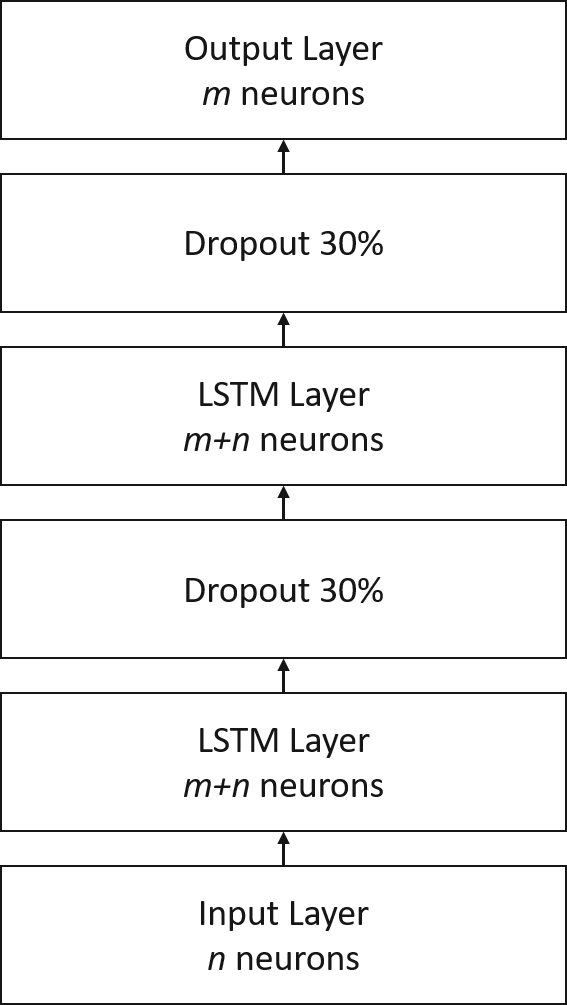
\includegraphics[width=0.3\textwidth]{gfx/schoenig-network-architecture.png}
    \label{fig:schoenig-architecture}
}
\caption{An overview of the reverse-engineered networks that are used as a comparison in this thesis.}
\label{fig:architectures}
\end{figure}

\begin{figure}
    \centering
    
\includegraphics[width=0.7\textwidth]{gfx/sp2-network-architecture.png}
    \caption{The SP2 and PFS networks share the architecture but inject different features.}
    \label{fig:sp2-pfs-architecture}
\end{figure}

Heavily inspired by these two architectures and the bipartite approach of Shibata et al. \cite{shibata2016bipartite}, Figures \ref{fig:sp2-pfs-architecture} present the injection of SP-2 or sub-sequence features at the top-level.

\section{Understanding a trace as a sequence}
The definition for sequences presented in \autoref{sec:background:sequence-prediction} needs to be extended so that a case trace can be understood as a sequence.

In the previous definition, the set $I$ had been used for \textit{items}, of which itemsets are comprised. An itemset represents a single row in the log. As such a row is made up of multiple different elements and adheres to a fixed schema, the definition needs to account for those two properties.\\

First, the set $I$ is now understood as a union of the sets $C_i$ which make up the distinct values inside one of the $n$ columns of a trace:
$$I = \bigcup\limits_{i=1}^{n} C_{i}$$

Second, each itemset $s$ needs to be bound by a specific schema. The schema needs to match the schema of the log and can be defined as such: $s = <i_1, i_2 ..., i_i>$ with $i_i \in C_i$. Thus, the original condition $s \subseteq I$ still holds true, but every item now has a fixed place in the itemset depending on which column it originates from.

\section{Evaluation criteria}
Three metrics of the four aforementioned implementations shall be the focus of the evaluation of the results:

\begin{enumerate}
    \item\textbf{Accuracy} - The share of total next-activity predictions.
    \item\textbf{Earliness} - Whether and how early the prediction accuracy begins to stabilize as the trace progresses; see Francescomarino~\cite{francescomarino2015}.
    \item\textbf{Feature importance} - Whether network-internal metrics indicate that an added feature is valuable for making predictions.
\end{enumerate}

While the first two criteria target the usability of the results, the last one permits making a judgment about the usefulness of the added features. This allows making a more informed decision about the necessity of the increased resource consumption.